%!TEX root = ../../root.tex


One fundamental limitation of autoencoders is their lack of guarantee about the regularity of the latent space.  Indeed, we could be tempted to think that, if the latent space is regular enough (well ``organized'' by the encoder during the training process), we could take a point randomly from that latent space and decode it to get a new content, acting as a \emph{generator}. However, it is pretty difficult (if not impossible) to ensure, a priori, that the encoder will organize the latent space in a smart way compatible with the generative process we just described. It could learn arbitrary functions, mapping similar inputs to arbitrarily distant regions of the latent space, without \emph{coupling}.

This weakness is addressed by \emph{Variational Autoencoders}, or \emph{VAE} in short. A VAE does not learn a mapping from the data space to the latent space and its ``inverse'', but explicitly constructs the parameters of a \emph{probability distribution} in the latent space, from which the latent codes are sampled.
\begin{figure}[H]
	\centering
	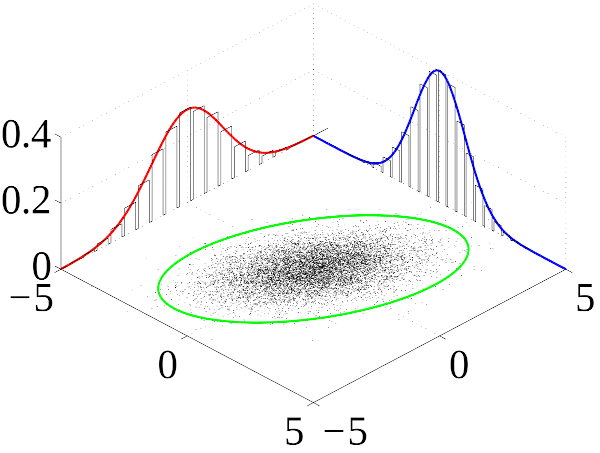
\includegraphics[width=.5\textwidth]{11/gauss}
	\caption{Variational Autoencoders with a multivariate Gaussian distribution.}\label{fig:gauss_variationalAE}	
\end{figure}
The form of the distribution is fixed and decided \emph{a priori}, for instance in the figure above we have chosen to represent the distribution of a $2$-dimensional code $\vb{z}$ as a (multivariate) Gaussian.
 
For what follows, it is nice to have some recap on \emph{information theory}: one is available at \cref{sec:appendix-A}.

The encoder is not a deterministic parametric function anymore, but is a \emph{probabilistic} parametric function, that models the parametric posterior distribution of the latent code $\vb{z}$, given the data $\vb{x}$
\begin{equation}
    \overbrace{p_\mathbf{\theta}(\mathbf{z} | \mathbf{x})}^{\mathclap{\text{probabilistic encoder}}} = \frac{p_\mathbf{\theta}(\mathbf{x} | \mathbf{z})p_\mathbf{\theta}(\mathbf{z})}{\underbrace{p_\mathbf{\theta}(\mathbf{x})}_{\mathclap{\text{prior on the input data}}}} = \frac{p_\mathbf{\theta}(\mathbf{x}, \mathbf{z})}{p_\mathbf{\theta}(\mathbf{x})}.
    \label{eq:prob_enc}
\end{equation}
This function is not deterministic since given the same input $\vb{x}$ twice, its output will not be the same $\vb{z}$, but rather it will be \emph{sampled} from the parametric distribution that it encodes. In fact, one often says that the function ``computes'' the distribution.

To compute \cref{eq:prob_enc}, i.e. have a computable expression for the encoder, we need to be able to compute the prior on the input data $p(\mathbf{x})$, i.e. how the input data is distributed. However, the following expression
\begin{equation}
	p_\mathbf{\theta}(\mathbf{x}) = \int p_\mathbf{\theta}(\mathbf{x} | \mathbf{z})p_\mathbf{\theta}(\mathbf{z})d\mathbf{z}
\end{equation}
is a high-dimensional, \emph{intractable} integral over all possible (continuous!) $\mathbf{z}$. 

Since we cannot exactly compute this term, it seems like we cannot compute \cref{eq:prob_enc} either. Indeed, the idea of variational autoencoders is to compute some approximation of that posterior distribution:
\begin{equation}
	q_\mathbf{\phi}(\mathbf{z} | \mathbf{x}) \approx p_\mathbf{\theta}(\mathbf{z} | \mathbf{x})
\end{equation}
where $q_\mathbf{\phi}(\mathbf{z} | \mathbf{x})$ is again a parametric probability distribution, with a \emph{fixed} form, and will depend on the parameters $\mathbf{\phi}$ of the neural network implementing the encoder.

Since we are looking for an approximation to $p$, we are going to ask that $q$ and $p$ are similar in the $KL$ sense \cref{eq:KL-divergence}, i.e. they have the same \emph{information content}. So we compute an approximation 
\begin{equation}
    q_{\mathbf{\phi}^*}(\mathbf{z} | \mathbf{x}) \approx p_\mathbf{\theta}(\mathbf{z} | \mathbf{x})    
\end{equation}
where $\phi^*$ is such that
\begin{equation}\label{eq:opt_prob_enc}
	\mathbf{\phi}^* = \argmin_{\mathbf{\phi}, \mathbf{\theta}} KL(q_{\mathbf{\phi}}(\mathbf{z} | \mathbf{x}) \| p_\mathbf{\theta}(\mathbf{z} | \mathbf{x})).
\end{equation} 

Once we obtain such a $\phi^*$, we have the expression for our encoder. However, at the moment we cannot even write down a closed form expression for \cref{eq:opt_prob_enc} as $p_\mathbf{\theta}(\mathbf{z} | \mathbf{x})$ is not given. However, with a somewhat long derivation we can simplify things:
\begin{align}
	\mathbf{\phi}^* &= \argmin_{\mathbf{\phi}, \mathbf{\theta}} KL(q_{\mathbf{\phi}}(\mathbf{z} | \mathbf{x}) \| p_\mathbf{\theta}(\mathbf{z} | \mathbf{x})) \\
	&= \argmin_{\mathbf{\phi}, \mathbf{\theta}} - \sum_{\mathbf{z}}q_\mathbf{\phi}(\mathbf{z} | \mathbf{x})\log \frac{p_\mathbf{\theta}(\mathbf{z} | \mathbf{x})}{q_\mathbf{\phi}(\mathbf{z} | \mathbf{x})} \tag{substituing the definition of KL} \\
	&= \argmin_{\mathbf{\phi}, \mathbf{\theta}} - \sum_{\mathbf{z}}q_\mathbf{\phi}(\mathbf{z} | \mathbf{x})\log \frac{p_\mathbf{\theta}(\mathbf{x}, \mathbf{z})}{q_\mathbf{\phi}(\mathbf{z} | \mathbf{x})} \frac{1}{p_\mathbf{\theta}(\mathbf{x})} \tag{substituing the definition of p}
\end{align}
Applying some properties of the logarithms we have:
\begin{align}
	\mathbf{\phi}^* &= \argmin_{\mathbf{\phi}, \mathbf{\theta}} - \sum_{\mathbf{z}} q_\mathbf{\phi}(\mathbf{z} | \mathbf{x}) \left(\log \frac{p_\mathbf{\theta}(\mathbf{x}, \mathbf{z})}{q_\mathbf{\phi}(\mathbf{z} | \mathbf{x})} + \log \frac{1}{p_\mathbf{\theta}(\mathbf{x})} \right) \\
	&= \argmin_{\mathbf{\phi}, \mathbf{\theta}} - \sum_{\mathbf{z}} q_\mathbf{\phi}(\mathbf{z} | \mathbf{x}) \left(\log \frac{p_\mathbf{\theta}(\mathbf{x}, \mathbf{z})}{q_\mathbf{\phi}(\mathbf{z} | \mathbf{x})} - \log p_\mathbf{\theta}(\mathbf{x}) \right)
\end{align}
Splitting the summation we obtain:
\begin{align}
	\mathbf{\phi}^* &= \argmin_{\mathbf{\phi}, \mathbf{\theta}} - \sum_{\mathbf{z}} q_\mathbf{\phi}(\mathbf{z} | \mathbf{x}) \log \frac{p_\mathbf{\theta}(\mathbf{x}, \mathbf{z})}{q_\mathbf{\phi}(\mathbf{z} | \mathbf{x})} + \sum_{\mathbf{z}} q_\mathbf{\phi}(\mathbf{z} | \mathbf{x}) \log p_\mathbf{\theta}(\mathbf{x}) \\
	&= \argmin_{\mathbf{\phi}, \mathbf{\theta}} - \sum_{\mathbf{z}} q_\mathbf{\phi}(\mathbf{z} | \mathbf{x}) \log \frac{p_\mathbf{\theta}(\mathbf{x}, \mathbf{z})}{q_\mathbf{\phi}(\mathbf{z} | \mathbf{x})} + \log p_\mathbf{\theta}(\mathbf{x}) \sum_{\mathbf{z}} q_\mathbf{\phi}(\mathbf{z} | \mathbf{x}) \\
	&= \argmin_{\mathbf{\phi}, \mathbf{\theta}} - \sum_{\mathbf{z}} q_\mathbf{\phi}(\mathbf{z} | \mathbf{x}) \log \frac{p_\mathbf{\theta}(\mathbf{x}, \mathbf{z})}{q_\mathbf{\phi}(\mathbf{z} | \mathbf{x})} + \log p_\mathbf{\theta}(\mathbf{x}) \tag{since the sum over all the z is equal 1}
\end{align}
Because minimizing a function is equivalent to maximizing the negative of that function:
\begin{equation}
	\mathbf{\phi}^* = \argmax_{\mathbf{\phi}, \mathbf{\theta}} \sum_{\mathbf{z}} q_\mathbf{\phi}(\mathbf{z} | \mathbf{x}) \log \frac{p_\mathbf{\theta}(\mathbf{x}, \mathbf{z})}{q_\mathbf{\phi}(\mathbf{z} | \mathbf{x})} - \log p_\mathbf{\theta}(\mathbf{x})
\end{equation}
Now, until now we have not solved anything, since the term $ \log p_\mathbf{\theta}(\mathbf{x})$ is still an intractable term. However, it can be proven that the summation is always smaller than $\log p_\mathbf{\theta}(\mathbf{x})$, i.e. it is a \emph{lower bound} for that term. Basically, since we are maximizing the function, the most we can do is \emph{tightening the gap} between the two terms, i.e. maximize the lower bound, so we relax the maximization problem and obtain:
\begin{equation}
	\mathbf{\phi}^* = \argmax_{\mathbf{\phi}, \mathbf{\theta}} \sum_{\mathbf{z}} q_\mathbf{\phi}(\mathbf{z} | \mathbf{x}) \log \frac{p_\mathbf{\theta}(\mathbf{x}, \mathbf{z})}{q_\mathbf{\phi}(\mathbf{z} | \mathbf{x})}
\end{equation}
The sum is known as \emph{Evidence variational Lower BOund}, so we can write:
\begin{equation}
	\mathbf{\phi}^* = \argmax_{\mathbf{\phi}, \mathbf{\theta}} ELBO_{\mathbf{\phi}, \mathbf{\theta}}(\mathbf{x})
\end{equation}
where 
\begin{equation}
	ELBO_{\mathbf{\phi}, \mathbf{\theta}}(\mathbf{x}) = \sum_{\mathbf{z}} q_\mathbf{\phi}(\mathbf{z} | \mathbf{x}) \log \frac{p_\mathbf{\theta}(\mathbf{x}, \mathbf{z})}{q_\mathbf{\phi}(\mathbf{z} | \mathbf{x})} \leq \log p_\mathbf{\theta}(\mathbf{x})
\end{equation}

Let's now see how to maximize this term:
\begin{align}
	&\max_{\mathbf{\phi}, \mathbf{\theta}} ELBO_{\mathbf{\phi}, \mathbf{\theta}}(\mathbf{x}) \\
	= &\max_{\mathbf{\phi}, \mathbf{\theta}} \sum_{\mathbf{z}} q_\mathbf{\phi}(\mathbf{z} | \mathbf{x}) \log \frac{p_\mathbf{\theta}(\mathbf{x}, \mathbf{z})}{q_\mathbf{\phi}(\mathbf{z} | \mathbf{x})} \\
	= &\max_{\mathbf{\phi}, \mathbf{\theta}} \sum_{\mathbf{z}} q_\mathbf{\phi}(\mathbf{z} | \mathbf{x}) \log \frac{p_\mathbf{\theta}(\mathbf{x}|\mathbf{z})p_\mathbf{\theta}(\mathbf{z})}{q_\mathbf{\phi}(\mathbf{z} | \mathbf{x})}
\end{align}
Again, using some logarithms properties and dividing the summation we gain:
\begin{align}
	&\max_{\mathbf{\phi}, \mathbf{\theta}} \sum_{\mathbf{z}} q_\mathbf{\phi}(\mathbf{z} | \mathbf{x}) \left( \log p_\mathbf{\theta}(\mathbf{x}|\mathbf{z}) + \log\frac{p_\mathbf{\theta}(\mathbf{z})}{q_\mathbf{\phi}(\mathbf{z} | \mathbf{x})} \right) \\
	= &\max_{\mathbf{\phi}, \mathbf{\theta}} \sum_{\mathbf{z}} q_\mathbf{\phi}(\mathbf{z} | \mathbf{x}) \log p_\mathbf{\theta}(\mathbf{x}|\mathbf{z}) + \sum_{\mathbf{z}} q_\mathbf{\phi}(\mathbf{z} | \mathbf{x}) \log\frac{p_\mathbf{\theta}(\mathbf{z})}{q_\mathbf{\phi}(\mathbf{z} | \mathbf{x})} 
\end{align}
The first term is just the expected value of $\log p_\mathbf{\theta}(\mathbf{x}|\mathbf{z})$ wrt $\vb{z} \sim q_\mathbf{\phi}(\mathbf{z} | \mathbf{x})$, while the second term represents a KL divergence, so we can write the previous equation as follows:
\begin{equation}\label{eq:var_enc_loss}
	\max_{\mathbf{\phi}, \mathbf{\theta}} \underbrace{\mathbb{E}_{\vb{z} \sim q_\mathbf{\phi}(\mathbf{z}|\mathbf{x})} \log p_\mathbf{\theta}(\mathbf{x}|\mathbf{z})}_{\mathclap{\text{likelihood of } \vb{x} \text{ given } \vb{z}}} - \underbrace{KL\left( q_\mathbf{\phi}(\mathbf{z} | \mathbf{x}) \| p_\mathbf{\theta}(\mathbf{z}) \right)}_{\mathclap{\text{ensures } q_{\phi}(\vb{z} | \vb{x}) \approx p_{\theta}(\vb{z})}}.
\end{equation}
In this expression, also the other part of the architecture, the \emph{decoder} shows up. In fact, the first term can be thought of as the goodness of the \emph{decoder}, since it is the likelihood of a datapoint given a latent code $\vb{z}$ sampled by the distribution modeled by the \emph{encoder} $q_{\phi}(\vb{z} | \vb{x})$.
 
On the other hand, the KL divergence term is what distinguishes VAEs from regular autoencoders. It ensures that the probabilistic encoder follows the distribution $p_\mathbf{\theta}(\mathbf{z})$. Wait, but $\theta$ are the parameters of the posterior, so what is $p_\mathbf{\theta}(\mathbf{z})$? In principle, it is the parametric prior over the latent codes $\vb{z}$, i.e. the distribution of the latent space. In practice, it is \emph{not} parametric, since we have said in the beginning that we would have fixed the latent space distribution, and here is where we fix it.

Usually, one chooses to have the prior over the latent space to be a (multivariate) \emph{Gaussian} with \emph{no free parameters}, so we remove $\theta$:
\begin{equation}
    p_{\theta}(\vb{z}) = p (\vb{z}) = \mathcal{N}_{\vb{0}, \vb{I}} (\vb{z}).
    \label{eq:11:3:prior-z}
\end{equation}
The idea is that the encoder will output some probability distribution over $\vb{z}$, that will be different for different datapoints $\vb{x}$, since it is a conditional probability. We will sample from this conditional probability to obtain an actual $\vb{z}$. Now, the KL term enforces that, \emph{regardless of} $\vb{x}$, this $\vb{z}$ should be distributed in the latent space like \cref{eq:11:3:prior-z}.

\begin{figure}[H]
	\centering
	\begin{overpic}
		[trim=0cm 0cm 0cm 0cm,clip,width=0.6\linewidth]{11/ae2}
		\put(-11,24){$\mathbf{x}\to$}
		\put(37,37.5){\footnotesize sample $\mathbf{z}$ from}
		\put(42,33){\footnotesize$\mathcal{N}(\bm{\mu},\bm{\sigma})$}
		\put(100,24){$\to\ell_{\pphi,\ttheta}$}
		%
		\put(12,23){\Large $\mathbf{q_\pphi(\mathbf{z} | \mathbf{x})}$}
		\put(66,23){\Large $\mathbf{p_\ttheta(\mathbf{x}|\mathbf{z})}$}
	\end{overpic}
    \caption{Variational autoencoder. The code $\vb{z}$ is sampled from $\mathcal{N}(\bm{\mu},\bm{\sigma})$, where $\bm{\mu},\bm{\sigma}$ depend on the incoming datapoint $\vb{x}$ but globally follows $\mathcal{N}(\vb{0}, \vb{I})$.} 
    \label{fig:variational_ae}	
\end{figure}

Now, what expressions do the (probabilistic) encoder and decoder have? Up until now we have only said that they model probability distributions, but what exactly are they?

Somewhat confusing, the probabilistic encoder also generates a Gaussian distribution. \textbf{Beware}, it is \textbf{not} necessarily equal to the prior $p(\mathbf{z})$, since this is a \emph{conditional} distribution, and hence depends also on the data $\vb{x}$:
\begin{equation}\label{eq:small_gauss}
	q_\mathbf{\phi}(\mathbf{z} | \mathbf{x}) = \mathcal{N}_{\mathbf{\mu}, \mathbf{\sigma}}(\mathbf{z}).
\end{equation}
In practice, the encoder produces the Gaussian mean $\mathbf{\mu}$ and variance $\mathbf{\sigma}$ as a function of the input $\mathbf{x}$ and the network parameters $\mathbf{\phi}$, and then those are used to explicitly generate the distribution to sample $\vb{z}$ from. Notice, once again, that this distribution is conditional, since it depends on $\vb{x}$. Different regions of the latent space will correspond to different ``types'' of datapoints. Suppose we have two points $\vb{x}_1, \vb{x}_2$: 
\begin{itemize}
    \item for $\vb{x}_1$ the probabilistic encoder will generate a pair of parameters $\vb*{\mu}_1, \vb*{\sigma}_1$, defining a conditional Gaussian $\mathcal{N}_{\vb*{\mu}_1, \vb*{\sigma}_1}(\vb*{z})$, and the various $\vb{z}_1$ we could sample from that Gaussian will be centered at the point $\vb*{\mu}_1$ and vary in a certain small region around it, with variance $\vb*{\sigma}_1$;
    
    \item for $\vb{x}_2$ the probabilistic encoder will generate a pair of parameters $\vb{\mu}_2, \vb{\sigma}_2$, defining a conditional Gaussian $\mathcal{N}_{\vb*{\mu}_2, \vb*{\sigma}_2}(\vb*{z})$, and the various $\vb{z}_2$ we could sample from that Gaussian will be centered at a \emph{different} point $\vb*{\mu}_2$ and vary in a certain \emph{different} small region around it, with variance $\vb*{\sigma}_2$.
\end{itemize}
 However, both the codes $\vb{z}_1$ and the codes $\vb{z}_2$ should be distributed, \emph{regardless} of what conditional Gaussian produced them and hence regardless of the input $\vb{x}$, like $p(\vb{z}) = \mathcal{N}_{\vb{0}, \vb{I}}(\vb{z})$.

\paragraph{VAE: Training}
Now, to actually train a VAE, since we usually minimize loss functions instead of maximize objective functions, we put a minus sign in front of \cref{eq:var_enc_loss} to get the \emph{loss function of VAEs}:
\begin{equation}
	\ell_{\mathbf{\phi}, \mathbf{\theta}} = - \underbrace{\mathbb{E}_{q_\mathbf{\phi}(\mathbf{z}|\mathbf{x})} \log p_\mathbf{\theta}(\mathbf{x}|\mathbf{z})}_{\mathclap{\text{reconstruction error}}} + \underbrace{KL\left( q_\mathbf{\phi}(\mathbf{z} | \mathbf{x}) \| p(\mathbf{z}) \right)}_{\mathclap{\text{regularizer}}}.
\end{equation}
The first term of the loss function represents the \emph{reconstruction error}, just like in the regular autoencoder case; the second term represents the novelty of VAEs, a \emph{regularizer} that enforces a prior on the distribution for the latent space thus enforcing  smoothness and compactness in the learned space, so that the chart from the Euclidean space to the manifold of the data, learnt by the decoder, should be continuous even in regions of the latent space that are not encountered during training.

\begin{figure}[H]
	\centering
	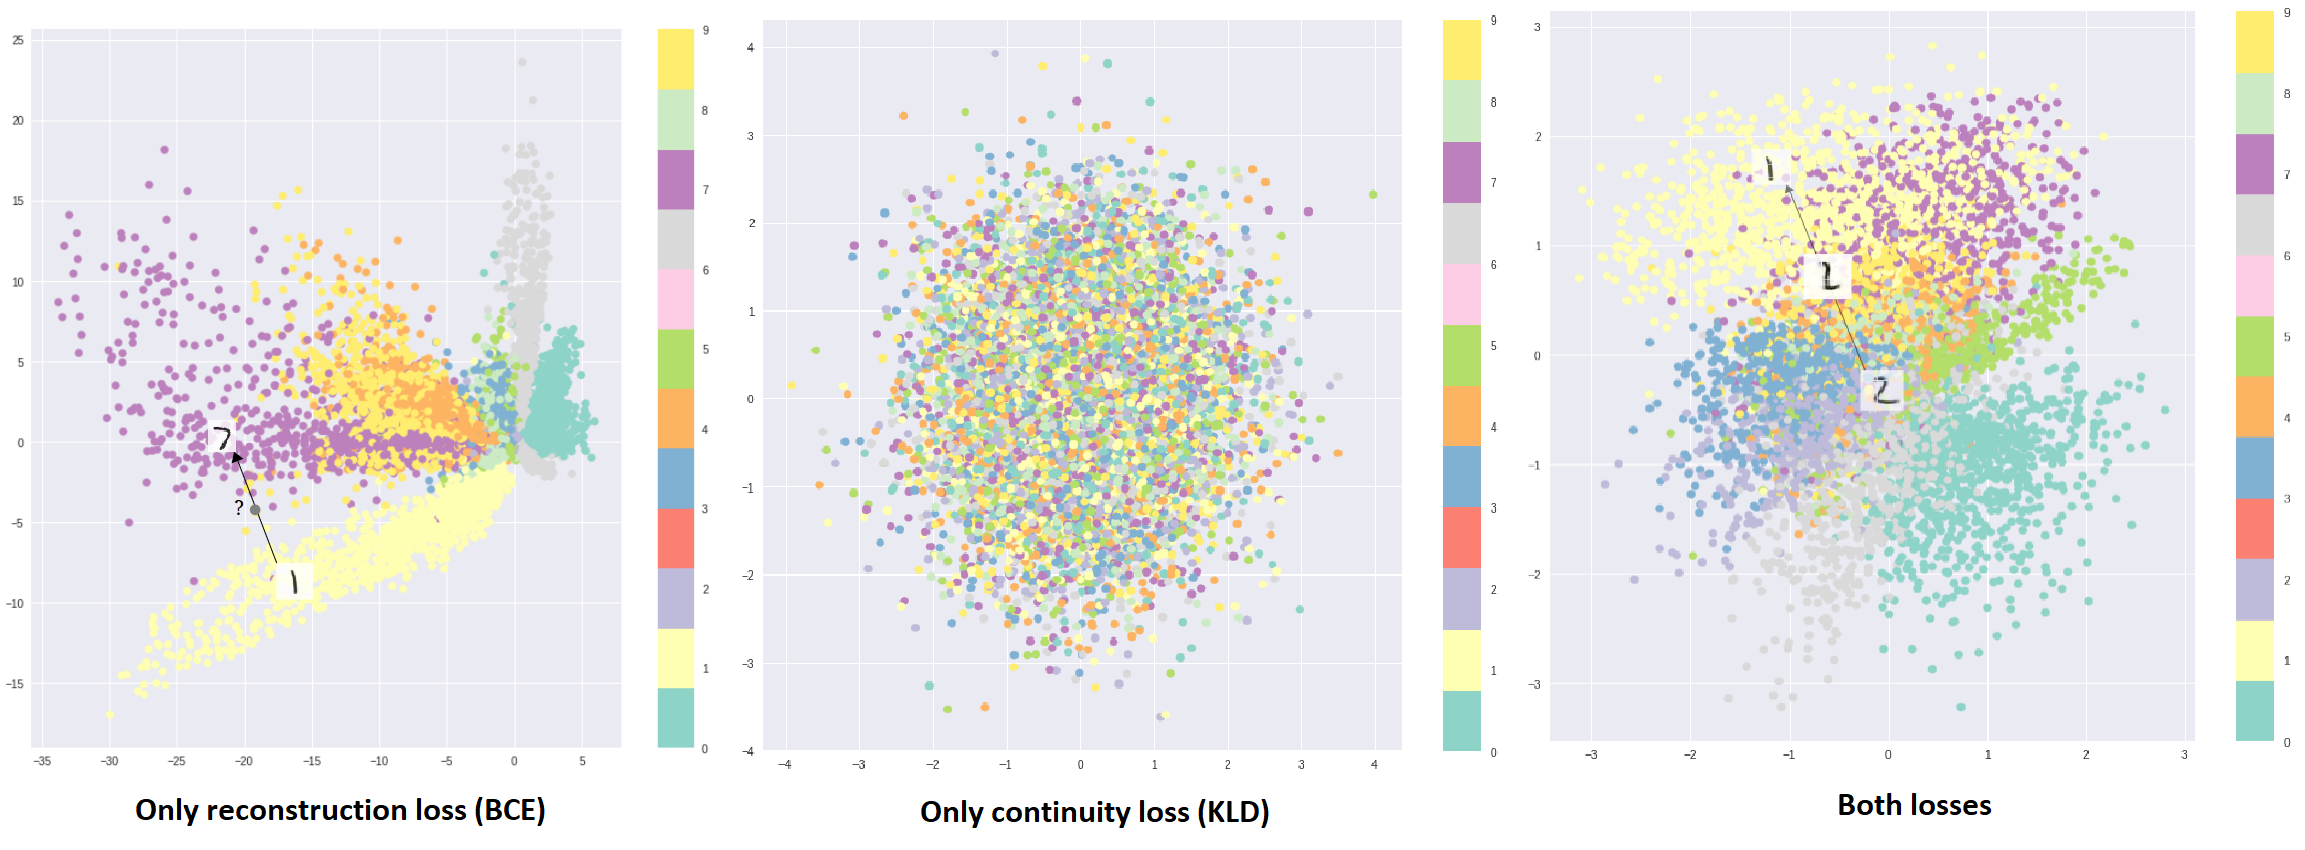
\includegraphics[width=\textwidth]{11/antonio}
	\caption{The role of the regularizer in VAEs, on the MNIST dataset. On the left we have no regularization, so regular autoencoders, in which the latent space is well behaved only in regions in which codes were assigned to observed data. In the center, only the regularization, so the codes are globally distributed as a normal Gaussian, but there is no correspondance with the input data, so we see codes for a digit mixed with codes for another digit. On the right, the combination of the two gives raise to a compact, smoothly changing distribution that has also localized regions (\emph{modes}) corresponding to certain digits.}\label{fig:regularizer_vae}	
\end{figure}

Note that the fact we are using two Gaussian distributions (in \cref{eq:11:3:prior-z} and in \cref{eq:small_gauss}) allows us to have a closed form expression for the regularizer\footnote{See \url{https://arxiv.org/pdf/1907.08956.pdf} for the expression and its derivation.}, and hence to write the loss in closed form.

When we train a VAE, the probabilistic encoder will ``output'' distributions $\mathcal{N}_{\mathbf{\mu}, \mathbf{\sigma}}$ from which we should sample to get a latent code to feed to the decoder. Recall that to train with a gradient descent-like algorithm we need to be able to backpropate gradients through the newtork, but this is a a problem, since in its naive form sampling from a random distribution is \emph{not} a differentiable operation. Since we are sampling at training time we need the sampling procedure be differentiable because we need to backpropagate through the network. 

To overcome this inconvenience, something called \emph{reparametrization trick} is employed, that makes the sampling procedure differentiable. The idea is that in the computational graph there is now a node (intermediate variable) $\vb{z}$ which is a \emph{random node}, something that backprop cannot flow through. However, we can make it so that $\vb{z}$ is not a \emph{source of randomness}, but is a \emph{deterministic function}
\begin{equation}
    \vb{z} = g_{\phi}(\vb{x}, \vb*{\epsilon}), \qquad \vb*{\epsilon} \sim p(\vb*{\epsilon})
\end{equation} 
that relies on an \emph{external source of randomness} $\vb*{\epsilon}$ . 

\begin{figure}[H]
    \centering
    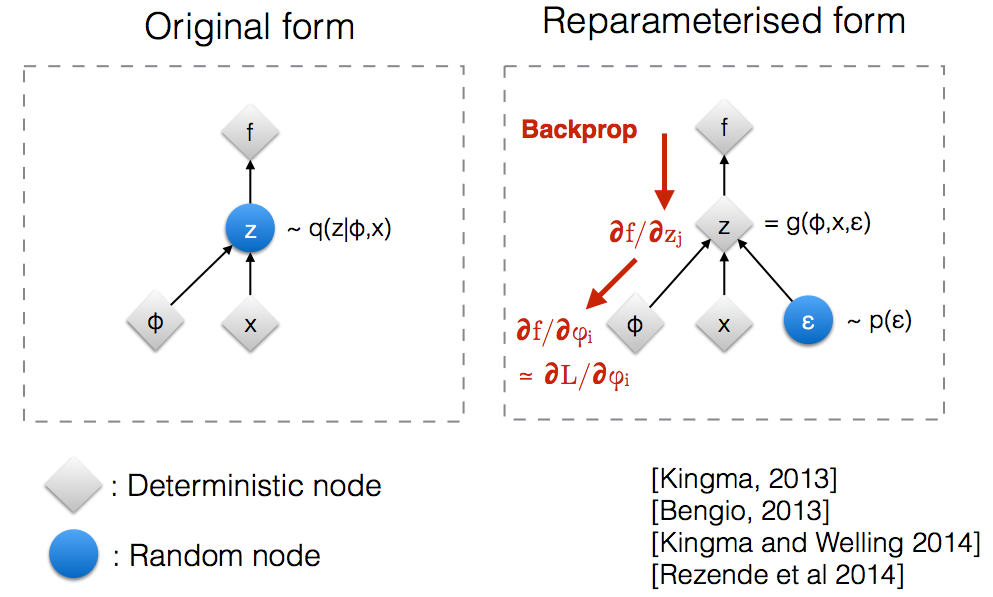
\includegraphics[width=.7\textwidth]{figures/11/rsample.png}
    \caption{Reparametrization trick.}
    \label{fig:11:3:rsample}
\end{figure}

Usually this function looks like
\begin{equation}
    \vb{z} = g_{\phi}(\vb{x}, \vb*{\epsilon}) = \vb*{\mu}_{\phi}(\vb{x}) + \underbrace{\vb*{\sigma}_{\phi} (\vb{x}) \odot \vb*{\epsilon}}_{\mathclap{\text{element-wise product}}}, \qquad \vb*{\epsilon} \sim \mathcal{N}(\vb{0}, \vb{I})
\end{equation}
where we are taking an external source of randomness that follows a normal Gaussian, sampling a value from it, then deterministically shifting it and rescaling it with the mean and variances computed by the encoder, get back a 
$$\vb{z} \sim \mathcal{N}_{\vb*{\mu}, \vb*{\sigma}}(\vb{z} | \vb{x})$$ 
in a \emph{deterministic} way. Where is the trick? We still need to sample from a distribution, something that is still not differentiable: there is still a random node in the computation graph. However, as you can see in \cref{fig:11:3:rsample} now we do \emph{not} need to backprop through this node, since the network parameters are on a different, separate path.

\paragraph{VAE: Testing}
When we are doing generation, we do not care about the encoding part of the VAE anymore and we only consider the decoder: we sample a latent code $\vb{z}$ according to \cref{eq:11:3:prior-z} and then we decode it to get a new, \emph{generated} sample $\vb{x}$.

However, sampling on the boundaries of the learned distribution can still lead to the generation of unlikely samples, since the VAE probably has seen few samples that were mapped to a latent code in that region, that is therefore poorly modeled.
\begin{figure}[H]
	\centering
	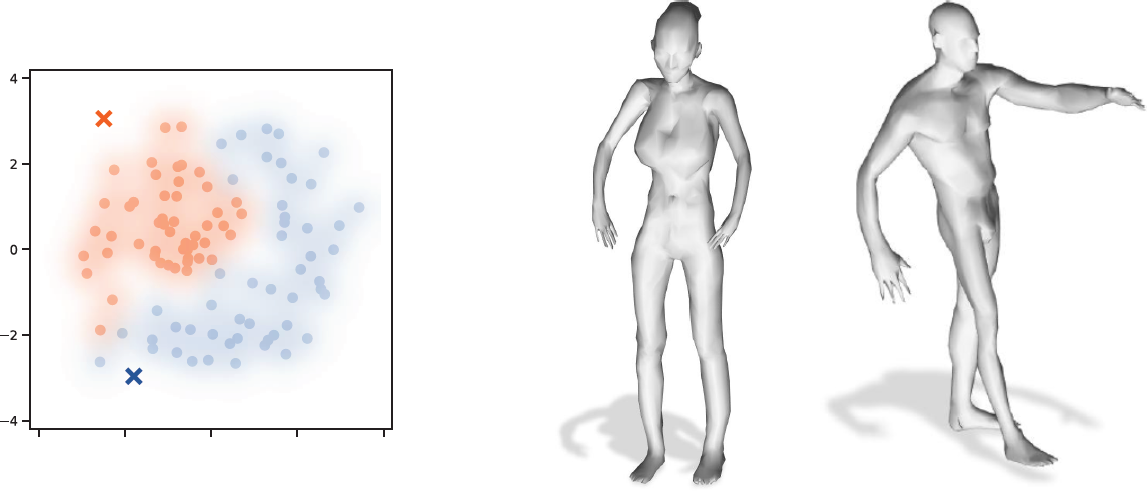
\includegraphics[width=.7\textwidth]{11/out}
	\caption{Sampling on the boundaries of the distribution.}\label{fig:unlikely_samples}	
\end{figure}

Another relevant phenomenon is \emph{posterior collapse}, in which the latents are ignored if the decoder becomes ``too powerful'', i.e. powerful enough to model the data perfectly, or if the encoder becomes ``too weak''. In fact, in this case $\vb*{\mu}$ and $\vb*{\sigma}$ collapse to some constant values $\vb{a}, \vb{b}$, so that
\begin{equation}
    q_{\phi}(\vb{z} | \vb{x}) \approx q_{\phi}(\vb{z}) = \mathcal{N}_{a, b}(\vb{z}),
\end{equation} 
the posterior of $\vb{z}$ \emph{collapses} to some fixed Gaussian, regardless of the input.
As a result, the decoder tries to reconstruct $\vb{x}$ by ignoring the uninformative $\vb{z}$ which are sampled from $\mathcal{N}_{a, b}(\vb{z})$.

\begin{minipage}{\textwidth}
\paragraph{VAE interpolation}
The regularity we induced in the latent space means that, once we have trained (correctly, which is hardly an easy task) a VAE, we can \emph{interpolate} between samples. This means choosing two samples ${\color{darkgreen}\mathbf{x}}_1, {\color{darkblue}\mathbf{x}}_2$, encode them to get their latent codes ${\color{darkgreen}\vb{z}}_1, {\color{darkblue}\vb{z}}_2$, and then trace a line between ${\color{darkgreen}\vb{z}}_1, {\color{darkblue}\vb{z}}_2$ and sample latent codes on the line. We are interpolating in the latent space, but if the decoder has correctly learnt a chart to the manifold of the data, by the continuity of the chart we should get samples that are close to the samples corresponding to the interpolating codes, effectively interpolating between samples. 
\begin{figure}[H]
	\centering
	\begin{overpic}
		[trim=0cm 0cm 0cm 0cm,clip,width=0.6\linewidth]{11/interp3}
		\put(-20,70){${\color{darkgreen}\mathbf{x}}_1\to$}
		\put(-20,35){${\color{darkblue}\mathbf{x}}_2\to$}
		\put(100,53){$\to$}
		\put(110,70){$\hat{\color{darkgreen}\mathbf{x}}_1$}
		\put(110,61){$\hat{\color{brown}\mathbf{x}}$}
		\put(110,52){$\hat{\color{pink}\mathbf{x}}$}
		\put(110,43.5){$\hat{\color{lightblue}\mathbf{x}}$}
		\put(110,35){$\hat{\color{darkblue}\mathbf{x}}_2$}
	\end{overpic}
	\caption{Variational Autoencoder interpolation.}\label{fig:interpolation}	
\end{figure}
\end{minipage}

If $\hat{\color{darkgreen}\mathbf{x}}_1, \hat{\color{darkblue}\mathbf{x}}_2$ were pictures of two digits generated by the decoder, the interpolated samples $\hat{\color{brown}\mathbf{x}}$, $\hat{\color{pink}\mathbf{x}}$, $\hat{\color{lightblue}\mathbf{x}}$ should be pictures of ``digits'' that resemble both.

\begin{figure}[H]
	\centering
	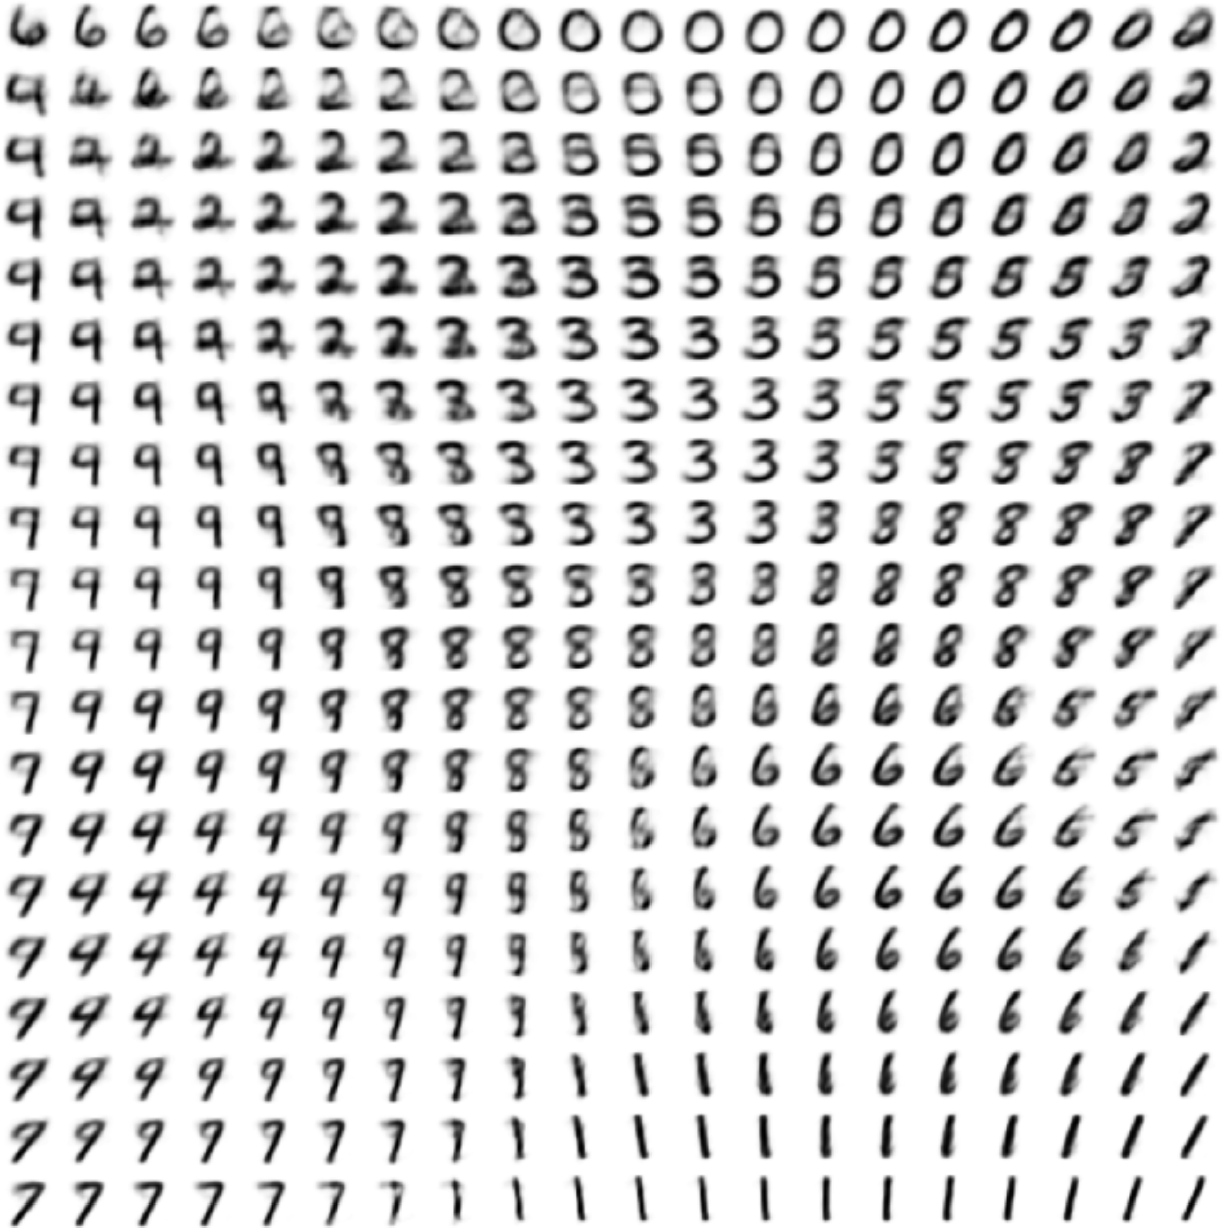
\includegraphics[width=.6\textwidth]{figures/11/mnist5.png}
	\caption{Interpolation between different images of digits.}\label{fig:interp-mnist}	
\end{figure}

Another interesting property of VAEs is that we can identify dimensions in the latent space that capture different semantics of the data, in particular we can do \emph{disentanglement}: for example in \cref{fig:disentanglement} one dimension represents the pose and the other dimension represents the identity of the person; then we can just interpolate along one dimension by setting a source point and a destination point and then change the dimensions spanning the expression. 

\begin{figure}[H]
	\centering
	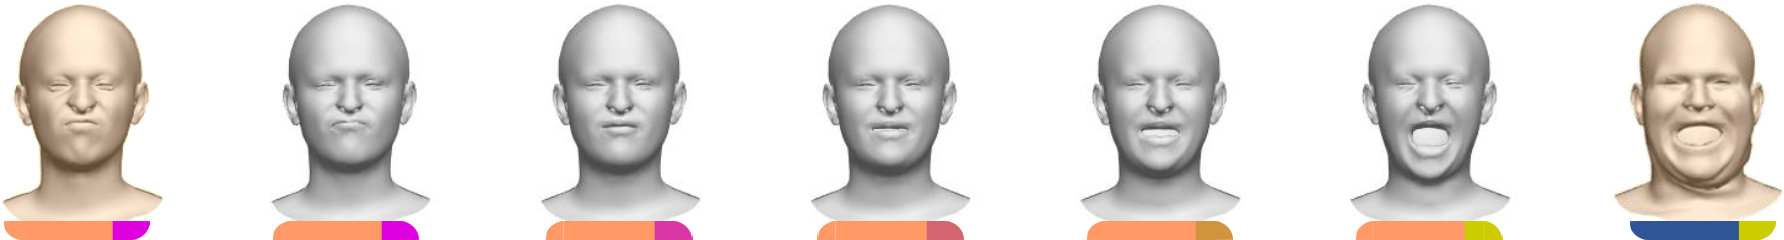
\includegraphics[width=.5\textwidth]{figures/11/faces3d.png}
	\caption{Disentaglement.}\label{fig:disentanglement}	
\end{figure}
